\chapter{Implementation} \label{ch:implementation}
\textcolor{red}{Summary}
\section{Overview}
This section provides an overview of the code structure and the datasets used in this project. The code is written in Python 3.10.10 , and uses PyTorch version 2.0.0. The entire codebase is available on \href{https://github.com/SubhadityaMukherjee/proxy_attention}{GitHub}. (As of now, the code is private, but will be made public after the evaluation is complete.) The entire requirements are listed in the \textit{requirements.txt} file in the root directory of the codebase. The structure of the codebase is shown in Figure ~\ref{fig:overview_code}.

A separate directory is used for each dataset, with each dataset being split into training and testing subdirectories. The results directory contains the aggregated runs, which are used directly in the report. The figures and tables are generated from the aggregated runs using the \textit{log\_viewer.ipynb} file. The runs directory contains the runs of the model. Each run has a folder with the run number, which contains the tensorboard logs and the checkpoints. 

The \textit{src} directory contains the source code for this project. The \textit{main.py} file is the entry point for the code and is used to configure the runtime hyperparameters. The \textit{proxyattention} folder contains the code for the model and the \textit{meta\_utils.py} file contains utilities that are reused across the codebase while the \textit{training.py} file contains all the code required for Proxy Attention and training the models.


\begin{figure}[H]
    \centering
    \begin{forest}
        for tree={
        font=\ttfamily,
        grow'=0,
        child anchor=west,
        parent anchor=south west,
        anchor=west,
        calign=first,
        edge path={
                \noexpand\path [draw, \forestoption{edge}] (!u.south west) +(7.5pt,0) |- (.child anchor)\forestoption{edge label};
            },
        before typesetting nodes={
                if n=1
                    {insert before={[,phantom]}}
                    {}
            },
        fit=band,
        before computing xy={l=15pt},
        }
        [Structure
            [Datasets
                    [Cifar100
                            [train]
                            [test]
                    ]
                    [dogs
                            [train]
                            [test]
                    ]
                    [\dots]
            ]
            [results
                    [aggregated\_runs.csv]
            ]
            [runs
                    [run001
                            [checkpoint]
                            [tensorboard logs]]
                    [\dots]
            ]
            [src
                    [proxyattention
                            [meta\_utils.py]
                            [training.py]
                    ]
                    [main.py]
            ]
        ]
    \end{forest}
    \caption{Code Directory Structure}
    \label{fig:overview_code}

\end{figure}


\section{Datasets}
To test Proxy Attention, a variety of datasets were chosen. The datasets were chosen to be of varying difficulty, and to have varying number of classes. The datasets used are \textbf{CIFAR100, Stanford Dogs, ASL Alphabet and Plant Disease dataset}. The datasets are described in detail in the following sections.

The images provided by the datasets are of varying sizes, but are resized to a similar size for consistency. These visualizations were generated by the author, and are not fully representative of the original dataset but are provided for reference. Due to space constraints, not all classes are shown in the visualizations. The complete list of classes and examples can be found in the links provided.

\subsection{CIFAR 100}
The CIFAR 100 dataset, introduced by \cite{krizhevskyLearningMultipleLayers}, is an image dataset with 60000 colour images with dimensions 32x32 pixels. As the name suggests, the dataset has 100 unique classes. Each of these classes has 500 training images. Some classes are - \textbf{airplane, bird, truck, ship, deer and dog}. This dataset is used as a coarse-grained classification dataset in this project.\\
The dataset and complete class information can be found \href{https://www.kaggle.com/datasets/fedesoriano/cifar100}{here}.

\begin{figure}[H]
    \centering
    \includegraphics[width=1\textwidth]{images/cifar100.pdf}
    \caption{A batch of images from the CIFAR100 dataset}
    \label{fig:cifar100}
\end{figure}

\subsection{Stanford dogs}
The Stanford Dogs dataset \cite{khoslaNovelDatasetFineGrained} is a popular fine-grained image classification dataset. There are more than 20k images in this dataset categorized into  120 classes of dog breeds like the \textbf{Afghan Hound , Appenzeller} etc. Being a fine-grained dataset, the images are very similar to each other and the classification task is much harder.\\
This dataset was chosen to further evaluate the explainability of Proxy Attention.\\
The dataset and complete class information can be found \href{http://vision.stanford.edu/aditya86/ImageNetDogs/}{here}.
\begin{figure}[H]
    \centering
    \includegraphics[width=1\textwidth]{images/dogs.pdf}
    \caption{A batch of images from the Stanford Dogs dataset}
    \label{fig:dogs}
\end{figure}


\subsection{ASL Alphabet}
The ASL dataset is a collection of hand pose images from the American Sign Language. There is no pose information with this dataset, but the images can be used for classification using the provided class labels.
The dataset chosen to evaluate Proxy Attention is the ASL Alphabet dataset, a more specific subset that has all the letters of the English alphabet along with the special characters \textbf{del, space and nothing}. The background is mostly the same, with minor changes. The data is also recorded from people with a similar skin tone, which makes the task easier.\\
This is an easy to classify dataset and was used as an initial test of the Proxy Attention mechanism. The results of the same are left in for future reference. \\
The dataset and complete class information can be found \href{https://www.kaggle.com/datasets/grassknoted/asl-alphabet}{here}.
\begin{figure}[H]
    \centering
    \includegraphics[width=1\textwidth]{images/asl.pdf}
    \caption{A batch of images from the ASL Alphabet dataset}
    \label{fig:asl}

\end{figure}

\subsection{Plant Disease}
This dataset consists of images of plant diseases across a variety of plants. The dataset is also a fine-grained classification dataset with 39 classes. Other than a few diseases, most of them are quite similar to each other, making the classification task harder. Some examples of the classes are \textbf{apple scab, blueberry healthy, cherry powdery mildew} etc.\\
The dataset and complete class information can be found \href{https://www.kaggle.com/datasets/rajibdpi/plant-disease-dataset}{here}.
\begin{figure}[H]
    \centering
    \includegraphics[width=1\textwidth]{images/plantdisease.pdf}
    \caption{A batch of images from the Plant Disease dataset}
    \label{fig:plant}

\end{figure}

\subsection{Caltech101}
The Caltech101 \cite{liCaltech101} dataset was created to tackle the absence of a uniform baseline comparison for vision classification tasks. The dataset has 101 categories of images, with a total of 9146 images. A background category is also included, which has images that do not belong to any of the 101 categories. An advantage of this dataset is that the images are of uniform size and have low clutter and occlusion, making it easier to classify. The caveat is that some categories have fewer samples than others.\\
The dataset and complete class information can be found \href{https://www.kaggle.com/datasets/862ae86edba271c39f76d0b530edeb55076b4b82b971160637210900747c44b1}{here}.
\begin{figure}[H]
    \centering
    \includegraphics[width=1\textwidth]{images/caltech101.pdf}
    \caption{A batch of images from the Caltech101 dataset}
    \label{fig:calt}
\end{figure}

\subsection{Places Dataset}
% - \cite{zhouPlaces10Million2018}
% - We release 2.5 million images from 205 scene categories to the public
% - This is a subset of the MIT places dataset consisting of 205 classes.
% - eg: engine room, excavation, kitchen
The Places dataset \cite{zhouPlaces10Million2018} contains 2.5 million images of different scenes. These scenes contain both indoor and outdoor scenes and have been categorized into 205 classes, including engine room, excavation, and kitchen. This dataset used for this research is a subset of the MIT places dataset, which comprises a total of 10\% out of the original 10 million images. The large-scale nature of the dataset allows for extensive exploration of scene recognition and understanding tasks but here it is used as a coarse-grained image classification dataset.\\
The dataset and complete class information can be found \href{https://www.kaggle.com/datasets/mittalshubham/images256}{here}.
% \begin{figure}[H]
%     \centering
%     \includegraphics[width=1\textwidth]{images/places.pdf}
%     \caption{A batch of images from the Places dataset}
%     \label{fig:places}
% \end{figure}


\subsection{Tsinghua Dogs}
% - \cite{zouNewDatasetDog2020}
% - Tsinghua Dogs is a fine-grained classification dataset for dogs, over 65\% of whose images are collected from people's real life. Each dog breed in the dataset contains at least 200 images and a maximum of 7,449 images, basically in proportion to their frequency of occurrence in China, so it significantly increases the diversity for each breed over existing dataset (see Fig. 1). Furthermore, Tsinghua Dogs annotated bounding boxes of the dog’s whole body and head in each image (see Fig. 2), which can be used for supervising the training of learning algorithms as well as testing them. 
% - Great Danes exhibit large variations in appearance, while (b) Norwich terriers and (c) Australian terriers are quite similar to each other.
The Tsinghua Dogs dataset \cite{zouNewDatasetDog2020} is a comprehensive fine-grained classification dataset specifically designed for dog breeds. It contains a substantial collection of images, with over 65\% of them collected from real-life sources. Each breed is represented by a minimum of 200 images and a maximum of 7,449 images. According to the authors, these values are somewhat proportionate to their relative population in China. This approach ensures increased diversity for each breed compared to existing datasets. The Tsinghua Dogs dataset also provides annotated bounding boxes for each dog's whole body and head in the images, for object detection tasks, but this information is not used for this project. With a wide range of breeds included, such as Great Danes and Norwich Terriers, the dataset exhibits significant variations in appearance. While some breeds are quite similar to each other, others are rather different, which further adds to the complexity of the image classification task. 
The dataset and complete class information can be found \href{https://cg.cs.tsinghua.edu.cn/ThuDogs/}{here}.

% \begin{figure}[H]
%     \centering
%     \includegraphics[width=1\textwidth]{images/tsing.pdf}
%     \caption{A batch of images from the Tsinghua Dogs dataset}
%     \label{fig:tsing}
% \end{figure}

\section{\textcolor{red}{Proxy Attention}}
- Let $I_{s} \in \mathbb{R}^{W \times H \times C}$ be a random source image
- applied saliency map $I_{vs}$ 
	- $I_{vs} = f(I_{s}) \in \mathbb{R}^{W \times H}$
	- Augmented image $I_{a}$
	- $\odot$ elementwise multi 
	- Mask $M \in \{0,1\}^{W \times H}$ 

% \begin{algorithm}
%     \caption{Single Batch Proxy Attention}
%     \label{alg:proxy_attention_single_batch}
%     \begin{algorithmic}
%         \REQUIRE $input\_wrong$
%         \REQUIRE $CAM$
%         \REQUIRE $proxy\_threshold$
%         \REQUIRE $proxy\_image\_weight$
%         \STATE $grads \leftarrow CAM(input\_wrong)$
%         \STATE $inversed\_normalized\_inputs \leftarrow inverse\_normalize(input\_wrong)$

%         \STATE $output \leftarrow REPLACE(grads \geq proxy\_threshold, ((1- proxy\_image\_weight) * grads) * inversed\_normalized\_inputs, inversed\_normalized\_inputs)$
%     \end{algorithmic}
% \end{algorithm}


% \begin{algorithm}
%     \caption{Batch Proxy Attention}
%     \label{alg:proxy_attention_batch}
%     \begin{algorithmic}
%         \REQUIRE $input\_wrong$
%         \REQUIRE $label\_wrong$
%         \REQUIRE $subset\_chosen$

%         \STATE $chosen\_inds = CEIL(subset\_chosen * LENGTH(input\_wrong))$
%         \STATE $input\_wrong\_subset = input\_wrong[:chosen_inds]$
%         \STATE $label\_wrong\_subset = label\_wrong[:chosen_inds]$

%         \STATE $processed\_labels \leftarrow [], processed\_thresholds \leftarrow []$
%         \FOR{$i \leftarrow 0$ \TO $LENGTH(label\_wrong\_subset)$}
%         \STATE $pass$ \#TODO
%         \ENDFOR

%     \end{algorithmic}
% \end{algorithm}

\section{Challenges and Potential Solutions}
Being a novel method, many challenges were faced while implementing Proxy Attention. While solving all the issues faced due to time constraints was not feasible, the author tried to tackle as many as possible. Many of these issues were posed as optimization problems and were considered hyperparameters that could be tuned to improve performance. This section discusses the possible solutions that were tested. Further details about each parameter can be found in Section ~\ref{sec:hyperparameters}.

\subsection{Proxy Method}
The Proxy Attention step involves replacing the pixels in the original images based on the attention maps obtained from a trained model. There are many different ways in which this can be done, some that were explored in the literature, some that were implemented and others that were left for future research. The following are the different methods that were considered:

\subsubsection{Image Statistics Based Replacement}
These methods use local or global statistical information from the images for replacement. All these methods can be computed per image, batch, or entire dataset.

\begin{enumerate}
    \item \textbf{Average Pixel Value}: The average pixel value of the original image is used for replacement.
    \item \textbf{Max Pixel Value}: The maximum pixel value of the original image is used for replacement.
    \item \textbf{Min Pixel Value}: The minimum pixel value of the original image is used for replacement.
    \item \textbf{0/255 Pixel Value}: The pixel value of 0 or 255 is used for replacement, where 0 refers to black and 255 refers to white.
\end{enumerate}
These methods are simple but naive, leading to significant information loss. In many cases, if many images have their values replaced with these values, the model might become biased towards predicting a specific class when an image contains many pixels with these values.
Due to this reason, these methods were not considered for the final implementation. A visualization of these methods can be found in Figure ~\ref{fig:methods}.

\subsubsection{Data Augmentation Based Replacement}
Data Augmentation techniques involve computing some transformation over images. Many of these methods were covered in the literature survey (Section ~\ref{sec:augmentation}), some of which replaced the pixels with random values, pixels sampled from either the current image or another image in the dataset, or even deleted the pixels. Most of these methods do not consider the model itself, but some, such as Saliency Mix \cite{uddinSaliencyMixSaliencyGuided2021} use saliency measures to find patches from other images in the dataset that are used to replace the chosen pixels.
These methods inspired Proxy Attention, but instead of replacing image patches or deleting pixels, it uses a gradient-based method to down-weight the pixels that might have led to the wrong prediction. This method moves away from using naive statistical information but enables the model to learn from its mistakes eventually.

\subsubsection{\textcolor{red}{GAN Based Replacement}}


\subsubsection{Modifying the Weights}
Instead of replacing the pixels, another possible method would be to modify the network weights directly. While many research papers elaborate on methods to perform this procedure, this domain still needs to be researched enough to be used easily. Research on this domain has been done from the early 90s \cite{schmidhuberSelfReferentialWeightMatrix1993}, but practical implementation of such a network that learns to modify its weight while training has not been extremely successful \cite{irieModernSelfReferentialWeight2022}.
That being the case, implementing such a method is left to future research.

\textcolor{red}{add some papers}

\subsubsection{Multiply with Attention Map}
The method chosen for this research does not directly replace the image's pixels but weights them using the attention map generated by passing the image through the trained model.
The obtained attention map is thus multiplied with the original image. In line with the principles of Proxy Attention, this allows the network to understand that the parts of the image it initially focused on did not lead to the correct result. Note that doing so is only possible if the network has seen this image. Because the images are slightly modified after the Proxy Attention step, if the network still needs to learn what the original image looks like, it might make more mistakes in the future by learning the wrong set of features.
A caveat of this method is that, after successfully applying the Proxy step to an image, the number of weighted pixels increases and, over time, might lead to the image not having any useful features left. This loss of information is tackled by clearing the proxy images every couple of steps.
A visualization of this method compared to others can be found in Figure ~\ref{fig:methods}.

\begin{figure}[h]
    \centering
    \includegraphics[width=1\textwidth]{images/methods.pdf}
    \caption{A comparison of different methods to replace the pixels in the original image}
    \label{fig:methods}
\end{figure}

\subsection{Training Biases}
Gradient-based XAI methods are not perfect, and in many cases, they are unable to provide accurate explanations for the predictions made by the model. Since Proxy Attention relies on the outputs of these methods, this might lead to the model learning biased representations of the data. This section discusses the different biases that might be introduced by using these methods in combination with Proxy Attention and how they can potentially be mitigated.

\subsubsection{Method Bias}
Not all explainability methods perform equally. Some methods are shown to have better masks generated, while other methods are more computationally expensive. Since Proxy Attention heavily depends on these methods, using them may lead to additional artefacts in the generated images. Some methods lead to better results while being used alongside Proxy Attention. To test the effects of this, multiple gradient-based methods are used to compare the performance of the networks.

\subsubsection{Mask Bias}
Proxy Attention uses the attention maps produced by gradient-based methods and multiplies them on the original image as a mask. While this works well, the masks themselves have edge artefacts that may lead to corrupting some regions of the image. These artefacts are further amplified for smaller image sizes and might impact performance in the long run.
Potential solutions include:

\begin{enumerate}
    \item Smoothing the masks before applying them to the image using techniques such as Eigen Smoothing. This could help in reducing the edge artefacts.
    \item Ensuring that only a certain percentage of the image is replaced by the Proxy Attention step. Doing so would preserve more information.
\end{enumerate}

\subsubsection{Learning Bias}

\begin{enumerate}
    \item Testing multiple schedules of when to apply the Proxy Attention step. This would help in understanding which part of the training process would benefit from the Proxy Attention step the most, reducing the computational overhead in the long run.
    \item Not reusing previously masked images for the Proxy Step. Doing so ensures that the artefacts are not propagated further into the training process.
\end{enumerate}

\subsection{Hyper Parameters} \label{sec:hyperparameters}
Proxy Attention is a novel method, and so there is no previous research on the best hyperparameters to use. The objective in choosing them is to find a balance between performance, computational overhead, and memory usage. The following section discusses the different hyperparameters that were tested and the reasoning behind their selection.

\subsubsection{Gradient Method}
Many gradient-based methods are available for generating attention maps from trained networks. While many of these methods were mentioned in the survey, it was impossible to test them all. Since Proxy Attention's effectiveness depends quite a bit on the gradient method used, it was important to test them.

The important factor considered while choosing these methods was the difference in complexity and the power of explanation they provide. While algorithms like GradCAM++ \cite{chattopadhayGradCAMGeneralizedGradientBased2018} provide more nuanced and better explanations of the image, older algorithms like Vanilla Gradients \cite{zeilerVisualizingUnderstandingConvolutional2013} are not so accurate. The objective here was to understand if using a more powerful method would improve performance with respect to classification accuracy when used with Proxy Attention. If this is the case, then it is possible to use more powerful methods to further improve performance in the future.
The gradient methods that were tested are as \textcolor{red}{follows}:
\begin{itemize}
    \item \textbf{GradCAM++} \cite{chattopadhayGradCAMGeneralizedGradientBased2018}.
    \item \textbf{GradCAM} \cite{selvarajuGradCAMVisualExplanations}
\end{itemize}

\subsubsection{Gradient Threshold}
Every gradient method considered generates a heatmap where the higher the activation, the more important the pixel is. The activations are mapped to a $[0,1]$ range with higher values in the heatmap indicating higher activation values. Since using Proxy Attention would mean that the pixels with the chosen activation values would be down-weighted, choosing a threshold value would result in the best classification accuracy was important.\\
This is a balancing act as choosing too small of a threshold would result in larger parts of the image being down-weighted, while choosing too large of a threshold would result in the image being down-weighted too little and hence being too close to the original image to make any difference.\\
A visualization of the different thresholds tested is shown in Figure \ref{fig:thresholds}.

\begin{figure}[H]
    \centering
    \includegraphics[width=0.8\textwidth]{images/grad_threshold.pdf}
    \caption{A visualization of the different thresholds and their effect on the image}
    \label{fig:thresholds}
\end{figure}

\subsubsection{Multiply Weight}
The Multiply Weight hyperparameter is used to control how strongly the attention map is applied to the image. The values are in the range $[0,1]$. A higher value would mean that the image is more strongly affected by the attention map, while a lower value would mean that the image is less affected. This is a balancing act as choosing too high of a value would mean that the image is affected too much, and important features might be lost from the image. Choosing too low of a value would mean that the image is not affected enough, rendering the Proxy step useless. The optimal value of this hyperparameter is found based on the results of the experiments conducted.

\textcolor{red}{generate and add figure here}

\subsubsection{Proxy Step Schedule}
Proxy Attention is a novel method, which means that there was no previous literature on how often to apply the Proxy step. To test this, multiple schedules were tested to understand how the network performs when the Proxy step is applied at different times.\\
The challenge faced while testing for this was that if the Proxy step was applied too many times, it might lead to overfitting, while if it was applied too few times, it might not have any effect. One might consider applying the Proxy step for every step, but this would be too computationally expensive. Since Proxy Attention also relies on the understanding of the model, applying the Proxy step too many times initially, when the network is not trained yet, might degrade performance as well.\\
These issues indicate a need for a schedule for the Proxy step as well. It is manually scheduled as of now, except when using the schedule generator (which is also a naive method).\\
Future work might include generating a schedule with respect to the validation accuracy. This might be a good idea as, if the network is not learning well, the Proxy step could be applied more often. But if the performance is already sufficient, then there remains no need to apply the Proxy step as frequently and potentially degrade performance.


\subsubsection{Subset Of Wrongly Classified}
This hyperparameter was chosen to understand if increasing the number of images that are passed to the Proxy step would help in improving performance. While providing more images might lead to better performance, the more images that are passed to the Proxy step, the more computationally expensive it becomes. To test this, both ends of the spectrum were tested, with a small fraction and a large fraction of the images being passed through the Proxy step.\\
As of now, the number of images passed to the Proxy step is taken as a fraction of the total number of images in the dataset. Future work could include a schedule for this as well, where the number of images passed to the Proxy step decreases over time as the network learns more and does not need as much help in improving performance.

\section{Data Loading and Pre-Processing}
Since many datasets were used in the project, it was important to ensure that the data was consistent across all the experiments.  Efficient use of memory and network performance were the main priorities while designing the data loading and pre-processing steps. This section details all the tweaks, custom loaders, and pre-processing steps that were used to ensure the same.

\subsection{Data Directory structure}
The data was stored in a specific directory structure similar to the ImageNet \cite{dengImageNetLargeScaleHierarchical2009} dataset to maintain consistency across the different experiments. Every dataset is divided into training and validation folders. Most of the datasets used in the project come with this split, but a validation split is created manually for those that do not. (Note that the test split is created from the training split while training the model and is not hardcoded.) For every class in the dataset, a subfolder within the parent folder is created with the name of the class.
All the datasets used are stored in the same folder on an SSD for ease of access and performance. The directory structure is shown in Figure ~\ref{fig:dataset_structure}.
\begin{figure}[H]
    \centering
    \begin{forest}
        for tree={
        font=\ttfamily,
        grow'=0,
        child anchor=west,
        parent anchor=south west,
        anchor=west,
        calign=first,
        edge path={
                \noexpand\path [draw, \forestoption{edge}] (!u.south west) +(7.5pt,0) |- (.child anchor)\forestoption{edge label};
            },
        before typesetting nodes={
                if n=1
                    {insert before={[,phantom]}}
                    {}
            },
        fit=band,
        before computing xy={l=15pt},
        }
        [Dataset
            [training
                    [image001]
                    [image002]
                    [\dots]
            ]
            [validation
                    [image001]
                    [image002]
                    [\dots]
            ]
        ]
    \end{forest}
    \caption{The structure of the Dataset Directory}
    \label{fig:dataset_structure}

\end{figure}

\subsection{Custom Data Loading}
A custom data loading logic was implementd for this project. The steps are as follows:
\begin{enumerate}
    \item First, the previously generated proxy images (if they exist) are cleared from the data folder. This is done to ensure that the proxy images are not loaded by mistake.
    \item For all the remaining images, the file paths are listed and shuffled.
    \item If the current step is a Proxy step, then for every proxy image loaded, the corresponding original image is not given to the data loader. This is done so that the number of images that the networks trained with and without Proxy Attention are equal.
    \item If the \lstinline[language=Python]{subset} parameter is set to a positive value, then only a subset of the data is obtained. If not, the entire dataset is used.
    \item Using these file paths, a Pandas DataFrame is created with the file path and label. The label is generated using a label function (Ref ~\ref{sec:label_function}) based on the file path.
    \item The labels are encoded and transformed into numerical values using the \lstinline[language=Python]{LabelEncoder} and \lstinline[language=Python]{LabelBinarizer} classes from the \lstinline[language=Python]{sklearn} library. A label map and reverse label map are created and stored in memory, a step that is useful for inference.
    \item To ensure an equal percentage of samples per class (some datasets used have unequal distributions), a Stratified K-Fold oversampling is applied.
    \item Before loading the images, an additional check is performed to ensure that the images have 3 channels. If they do not, then they are converted to RGB. This check is performed as some images in the datasets could be transparent, have 4 channels, or accidentally be grayscale. Not handling these images lead to errors while training and hence they are preemptively converted to RGB.
\end{enumerate}

\subsection{Label function} \label{sec:label_function}
To ensure easy compatibility with new datasets, label functions are used to obtain labels given a file path instead of hardcoding them. This enables a uniform API that can be extended to any dataset by writing a simple lambda function.\\
In the previous step, a Pandas DataFrame with the file paths of all the images was created. To generate labels, the label function is mapped across the entire column of file paths. This function is also used to create the label map and reverse label map, that is useful for inference.\\
For example, consider the ASL dataset. The file path for a single training image is of the form \begin{verbatim}
    /media/subhaditya/datasets/ASL/asl_alphabet_train/asl_alphabet_train/A/A1.jpg
\end{verbatim} To obtain the label, a lambda function
\lstinline[language=Python]{lambda x: x.split("/")[-2]}
is used.
The label function splits the string into a list by the Unix path label separator "/" and returns the second last element in the list. Thus, the label for this image becomes \textbf{A}.\\


\subsection{Clearing proxy images} \label{sec:clearing_proxy_images}
The images are saved locally for every iteration of the Proxy Attention step. That being the case, using these generated images over further iterations of the Proxy Attention step is possible. Since these images replace the original image from the data set, it is possible to use them as a direct substitute for the original images in the data set.  Note that doing so would give the network more images when using Proxy Attention during training, which is potentially an unfair comparison. Only a single image is chosen during the data loading process to avoid this issue. Thus, this becomes a hyperparameter where the options are either to store the last generated proxy images across iterations and use those images as direct replacements for the original images or not perform the step.

In the long run, the option to persist the images across iterations could lead to the network learning artefacts introduced in prior iterations. To make sure that the networks that train with Proxy Attention are fairly compared with the ones that do not, the data loader is only passed either the original image or its substitute but not both.

\subsection{Augmentations}
Augmentations are a useful step in training neural networks and increasing robustness to new data. Since this project is a test of Proxy Attention and not of improving performance of specific architectures, a minimal set of augmentations are used. All the transforms are applied using \textbf{torchvision}.\\
For both training and validation, the images are normalized using the ImageNet statistics. This is done to maintain a standard, and also since the pretrained models used have been trained on ImageNet \cite{dengImageNetLargeScaleHierarchical2009}. The mean and standard deviation used are \begin{verbatim}
    mean = [0.485, 0.456, 0.406]
    std = [0.229, 0.224, 0.225]
\end{verbatim}
For training, the images are resized to $224\times224$. Random horizontal flips are also applied with a probability of $0.5$ along with random rotations with a maximum angle of 10 degrees and a similar probability. The images are then converted to Tensors.\\
For validation, the images are resized to $224\times224$ and then converted to Tensors. No further augmentations are applied.\\

\section{Architectures}
This section discusses the architectures used and the library used to implement them.

\subsection{TIMM}
The library used to load the models is called \textbf{TIMM} \cite{wightmanRwightmanPytorchimagemodelsV02023}. It is a PyTorch library that provides a vast number of models with the option of loading pretrained versions of the same. The library also provides an easy way to customize the loading options for transfer learning, including the ability to choose the number of classes, the number of layers to freeze, Global Pooling options, etc.\\
The following models were used in this project:

\subsection{\textcolor{red}{ResNet - 18,50}}
- prev misconception : deeper the network, better performance ; but vanishing grads
- skip connections : loss of info
- act of n-1)th conv added to out of n+1)th ; adds relu, skips nth layer
- if nth layer doesnt learn, no information loss
- enabling the network to skip one ReLU activation in between if it does not provide any useful information or provides no information at all i.e, 0, and the network will be using the previous information, thus maintaining consistent performance
- If anyways both the layers are providing significant information, thus having previous information will anyways boost the performance.

\subsection{\textcolor{red}{VGG16}}
\subsection{\textcolor{red}{EfficientNetB0}}
\subsection{\textcolor{red}{ViT Base Patch $16\times224$}}

\section{Grid Search}
A grid search was performed to test the effectiveness of Proxy Attention and to find the best combination of hyperparameters. The grid search was performed on a single machine with a single GPU. An analysis script was written to determine what trials to run instead of using a separate optimization framework (Ref ~\ref{sec:result_aggregation}).
Due to limited resources, an initial sweep over the hyperparameters was performed using a low memory network (ResNet18 \cite{heDeepResidualLearning2016}), a subset of the Dogs dataset (\cite{khoslaNovelDatasetFineGrained}), a simple gradient method (GradCAM \cite{selvarajuGradCAMVisualExplanations}) and a small number of epochs. A separate process was started for each trial in the grid search, and the memory was cleared after each trial. This process was repeated until the best combination of hyperparameters was found. Once the worst-performing parameters were eliminated, the rest of the trials were run for the other networks, datasets and methods.
Although it was possible to use a separate optimization framework and an algorithm like Bayesian Optimization to find the best combination of hyperparameters, the parameters were semi-automatically chosen instead due to a lack of resources and time.

\section{Training Resumption}
Training resumption was an important part of this project. Since Proxy Attention is applied between training runs, it was important to be able to resume training from the last checkpoint. Furthermore, since a single machine was used, resuming broken trials easily was a useful feature to have. This section discusses the challenges faced in creating this feature and the solutions implemented to overcome them.

\subsection{Checkpoints} \label{sec:checkpoints}
While checkpoints are almost always a good idea, they were especially important in this project. The Proxy Attention step is applied between training runs, and to preserve memory, it unloads the existing models and DataLoaders from the GPU. This means that when continuing training, the models and DataLoaders need to be reloaded before the next training run. Doing so would effectively reset the training process, so it was important to have checkpoints to resume training.
As part of the final analysis, the author also iterated over the trained models and compared the explainability of models trained with or without Proxy Attention. Having saved checkpoints made this process much easier.

\subsection{Broken Trials}
A challenge of training on a single machine was that the training process could be interrupted at any time. Since this project required several experiments to find the best combination of hyperparameters, it was important to be able to resume training in case of any interruptions. The author initially tried using libraries such as \href{https://github.com/optuna/optuna}{Optuna} and \href{https://github.com/ray-project/ray}{Ray Tune}, but these added too much of an overhead for this project. (Ref ~\ref{sec:challenges_with_external_libraries}) A custom solution was implemented instead.\\
The objective of the solution was to be able to reload the last configuration and continue the training from there. In the implementation, the trials were generated as a list of possible configurations, and the program iterated over the list to run them. If the trial broke, the list of configurations and position of the current trial in the list was saved as a pickled dictionary. Using this saved object, the script could easily reload the last configuration and continue training without having to start from the beginning.\\
An additional useful feature of this solution was that it allowed the author to quickly patch any minor bugs without having to reiterate over the entire list of trials. This was especially useful when the author was testing the code for the first time and had to fix several bugs in the code.

\subsection{Challenges with External Libraries} \label{sec:challenges_with_external_libraries}
Some of the challenges that were faced while using external libraries are as follows:
\begin{enumerate}
    \item \textbf{GPU cache}: While Ray Tune and Optuna manage resources efficiently, they did not clear the GPU cache effectively. PyTorch, by default, holds on to the GPU cache and does not release it until the program is closed for efficiency. This would not be a problem for a single training run, but if many trials were being run, the cache would quickly fill up and cause the training to crash. This does not imply that using Proxy Attention makes it impossible to use such libraries but that it was easier to implement a custom solution.
    \item \textbf{Cluster} : Both libraries were written to enable running large-scale experiments over multiple machines. While this would be useful for a large-scale project, it added unnecessary complexity to this project as all the experiments were run on a single machine.
    \item \textbf{Grid Search} : Both libraries mentioned above were designed for hyperparameter tuning and to implement multiple grid search variants. While this would be useful, it would stop many trials that would eventually be useful to analyze. In this project, it was important to have results for each of the trials, and since the author could not find a way to disable the default Early Stopping behaviour as part of the grid search, a simple trial generation algorithm was created instead.
\end{enumerate}

\section{Optimizations}
The following section discusses the optimizations that were implemented to improve the performance of Proxy Attention, training the networks and reducing memory usage.

\subsection{Proxy Step specific}
The Proxy Attention step is the most computationally expensive step in the training process since it applies an XAI algorithm to each of the images in the batch of wrongly classified images. To reduce the time taken to apply the XAI algorithm, the following optimizations were implemented:
\begin{itemize}
    \item \textbf{CPU}: The CPU was used to store the wrongly classified images and labels as GPU memory is limited. The images and labels were stored during an epoch on the CPU and then passed to the GPU for the Proxy Attention step in batches.
    \item \textbf{Computational Graph}: The computational graphs of the wrongly classified images were deleted as they were not required and storing them unnecessarily increases memory usage.
    \item \textbf{Native PyTorch}: All computations were done on the GPU using PyTorch tensors, unlike many libraries that use numpy arrays. This reduced the overhead of converting between numpy arrays and PyTorch tensors and enabled the use of the GPU for all computations.
    \item \textbf{torch.where}: Replacing the pixels in the image was done using torch.where which is much faster than simply iterating over the image and replacing the pixels.
    \item \textbf{Freeing GPU memory}: The gradients were deleted from the GPU after the step was completed to reduce memory usage. This was done using \textit{del} and then calling \textit{torch.cuda.empty\_cache()} to free the memory.
    \item \textbf{Batching}: All preprocessing steps, label changes, etc., were done in batches to reduce memory usage and CPU calls.
    \item \textbf{Saving Images}: It is a known issue that saving images as \textit{png} files with no compression is slow using Pillow and thus the images were saved as \textit{jpeg} files instead. (Ref. ~\href{https://github.com/python-pillow/Pillow/issues/1211}{Github issue}). In practise, \textit{jpeg} images have smaller file sizes than \textit{png} images, which inturn reduces the additional storage required.

\end{itemize}

\subsection{Grid Search}
The major challenge with implementing a grid search was the memory usage. On a single machine, PyTorch reserves some memory for itself, and this memory is not released until the program is closed. This means that if the grid search is run sequentially, the memory usage will increase with each trial and eventually lead to a crash. The solution implemented was to run each trial as a separate process and call it from a main script. This ensured that the memory was released after each trial and the memory usage was kept in check.\\
This project did not require training multiple models simultaneously and so parallelization was not required or implemented.

\subsection{Workers}
By default, PyTorch uses a single worker to load data from the SSD. This is not ideal, as the resources must be fully utilized. The author used eight workers to load data from the SSD, which improved the training process's performance. Increasing the number of workers beyond a certain point does not necessarily improve performance due to the overhead of transferring data between the CPU and GPU and might lead to detrimental effects.

\subsection{Mixed Precision}
Mixed Precision Training \cite{micikeviciusMixedPrecisionTraining2017} involves computing most of the operations in the network in half-precision (16-bit) and only using full precision (32-bit) for important operations such as the loss function. This allows for much larger batch sizes, faster training, and reduced memory usage. Micikevicius et al. also find that using Mixed Precision training does not significantly affect the model's accuracy. With all these benefits, using Mixed Precision training was a no-brainer for this project.

The only caveat is that only some operations are stable in half precision. Operations like Batch Normalization tend to break when using Mixed Precision training, and unless managed, the model fails to converge. PyTorch supports \href{https://pytorch.org/docs/stable/notes/amp_examples.html}{automatic casting} to and from half-precision and this API was used for this project. It is also a registered issue that Transformer models sometimes fail to converge with Mixed Precision due to the way that Attention is calculated (Ref ~\href{https://github.com/pytorch/pytorch/issues/40497}{PyTorch Issue \#40497}), and so for the Vision Transformer \cite{dosovitskiyImageWorth16x162021} model, the author had to use full precision.

\subsection{No grad}
Since a single machine was used for training, it was important to reduce memory usage wherever possible. Since it was not necessary to store the gradients for the validation step as they are not used for anything, one of the ways to reduce memory consumption is to disable gradient computation for the validation step. This is done by using the \texttt{torch.no\_grad()} context manager.  The optimizer's \texttt{zero\_grad()} method is used to clear the gradients (using \texttt{set\_to\_none=True}). The additional parameter \texttt{set\_to\_none} is shown to have better performance (Refer to the ~\href{https://pytorch.org/tutorials/recipes/recipes/tuning_guide.html}{Official PyTorch tuning guide} for more information.) as it involves fewer operations.

\subsection{Pillow SIMD}
SIMD (Single Instruction, Multiple Data) is a computational technique that allows for the simultaneous execution of the same operation on multiple data points by utilizing multiple processing elements. It is particularly advantageous when compiled for specific processors, leading to improved performance in tasks such as graphics and image processing. SIMD operates synchronously and deterministically, making it suitable for operations that traditionally rely on the capabilities of a GPU. Since one of the major bottlenecks in the training process is loading images from the SSD, using SIMD operations is a way to reduce the latency. A few years ago the image processing library Pillow, used to be one of the majorly used libraries for loading images. In recent times, it has been superceded by the \href{https://github.com/uploadcare/pillow-simd}{Pillow SIMD} library, which uses SIMD instructions to improve performance. Pillow SIMD's API is a drop-in replacement for Pillow and requires no changes to the code but increases image I/O speeds by a significant margin (Refer to ~\href{https://python-pillow.org/pillow-perf/}{Benchmark comparison between Pillow and Pillow SIMD}).


\section{Tensorboard}
Tensorboard is a utility for managing and visualizing training logs. In this project, it is used to store the training configurations, metrics, images and other information that is generated during training. Since Tensorboard uses a custom file format to store this information, it can be used to store any information. Unlike many other logging utilities, Tensorboard stores all its logs locally. While storing them online might be useful in some cases, it is more difficult to manage and quite unnecessary for this project.
Another useful feature of Tensorboard is the ability to see live updates while training is in progress. This is useful for debugging and ensuring the training is progressing as expected.

\section{Optimizer}
While ADAM \cite{kingmaAdamMethodStochastic2014} is one of the most used optimizers in the deep learning community, Lonschiolov et al. \cite{loshchilovDecoupledWeightDecay2019} show that many libraries implement weight decay incorrectly. This finding was inspired by the choice of many researchers to use SGD with momentum instead of ADAM as it somehow seemed to perform better in many cases, but the reason for the difference in performance was not well understood. After finding the issue, Lonschiolov et al. proposed a simple fix to the weight decay implementation in ADAM, which they called ADAMW.

The error comes from the incorrect assumption that weight decay and L2 regularization are the same. While in the case of SGD, this indeed is the case, it is not true for other optimizers, especially ADAM. In the case of ADAM, WD first applies the update and then subtracts a portion of the weight. While L2 regularization adds the weight decay term to the gradients and then computes the moving average of the gradients and the corresponding squares before applying them to the update. Many of the deep learning libraries use L2 regularization instead of weight decay in their implementations, which leads to a significant difference in performance. Another important point to note is that the weight decay must be disabled for the optmizers as doing so will lead to L2 regularization being applied, which defeats the purpose of using ADAMW.
In this project, the ADAMW optimizer is used with a learning rate of $10^{-3}$ and a weight decay of $10^{-5}$.

\section{LR scheduler}
Choosing an appropriate learning rate is an important step when training a neural network. A learning rate that is too high might lead to the model overshooting the local minima when traversing the loss landscape. While a learning rate that is too low might lead to the model taking a long time to converge. A learning rate scheduler is used to find the optimal learning rate during training. The LR scheduler used in this project is the One Cycle LR scheduler proposed by Smith et al. \cite{smithSuperConvergenceVeryFast2018}.

In their paper, the authors propose a cyclic LR scheduler that moves from a lower LR to a higher LR in cycles. An LR finder is used to find the maximum LR that can be used for training. The LR finder is a simple algorithm that starts with a very low LR and increases it by a tiny amount for a number of iterations. If the loss starts to increase fast for the chosen LR, the LR finder terminates and the maximum LR is obtained. 
The One Cycle policy builds up on previous research done on warming up the learning rate at the beginning of training. While other approaches move directly to a higher LR after the initial warmup, Leslie et al. suggest a slower approach to the same. In the middle, the LR rizing can be thought of as a regularization method.

In addition to the cycle of LR, the authors also propose a cycle of momentum. They suggest that the momentum should be high at the beginning of training and should be decreased as the LR increases. This is because using a higher momentum at the beginning of training allows the model to quickly traverse the loss landscape and attempt to find local minima, but in later stages, a lower momentum is beneficial as it helps the model to converge to a local minima stably instead of overshooting it. Using a cyclic momentum removes some of the guess work involved in choosing the optimal momentum value for training, as the momentum is from lower to higher values in a cycle. 

Other benefits of the One Cycle Policy include the ability to use higher batch sizes and LRs, while also reducing the need for other regularization techniques due to the inherent regularization effect of the One Cycle Policy.

In this thesis, an LR finder is not used to find the maximum LR but set to $2\times 10^{-3}$ instead. While this is suboptimial, since the focus of this work was not to find the best performance, but just test the effects of Proxy Attention, this choice was made to reduce the number of hyperparameters that needed to be tuned. Future researchers should feel free to experiment with the LR finder to improve the accuracy further.

\section{Loss function}
The Cross Entropy Loss function is a popular loss function that is used in multi-class image classification tasks. Derived from the field of information theory, it uses the concept of entropy to quantifies the discrepancy between two given probability distributions. In this project, the Cross Entropy Loss is used for training the models. The formula for computing the loss is given by $\mathscr{l}(x,y) = L = \{l_{1}, ..., l_{N}\}^{T}$ where $l_{n} = -w_{y_{n}}log \frac{exp(x_{n, y_{n}})}{\Sigma_{c=1}^{C}exp(x_{n,c})}$, $x$ is the input, $y$ is the target, $C$ is the number of classes. By evaluating the predicted class probabilities against the ground truth labels, the loss function captures the dissimilarity between the predicted and actual class distributions. 

\section{Batch Size Finder}
To maximize training performance, a batch size finder (Ref ~\ref{fig:bsfinder}) is used to find the optimal batch size for each model.

The batch size finder algorithm is rather simple. It starts by testing for a small batch size of 2. This batch size is then successively, either incremented or decremented, based on the current GPU configuration's ability to support that batch of data.
A random batch of data with the size that is to be tested is generated and passed through the required model. If the GPU fails to accommodate the current batch of data, the loop terminates, and the required batch size is obtained. The rest of the steps required to train a network are also performed on this randomly generated data.
This algorithm remains the same for any model, data type, or other further optimizations applied (such as mixed precision training \cite{micikeviciusMixedPrecisionTraining2017}) and is robust to multiple GPUs being used for training.

\begin{figure}[H]
    \centering
    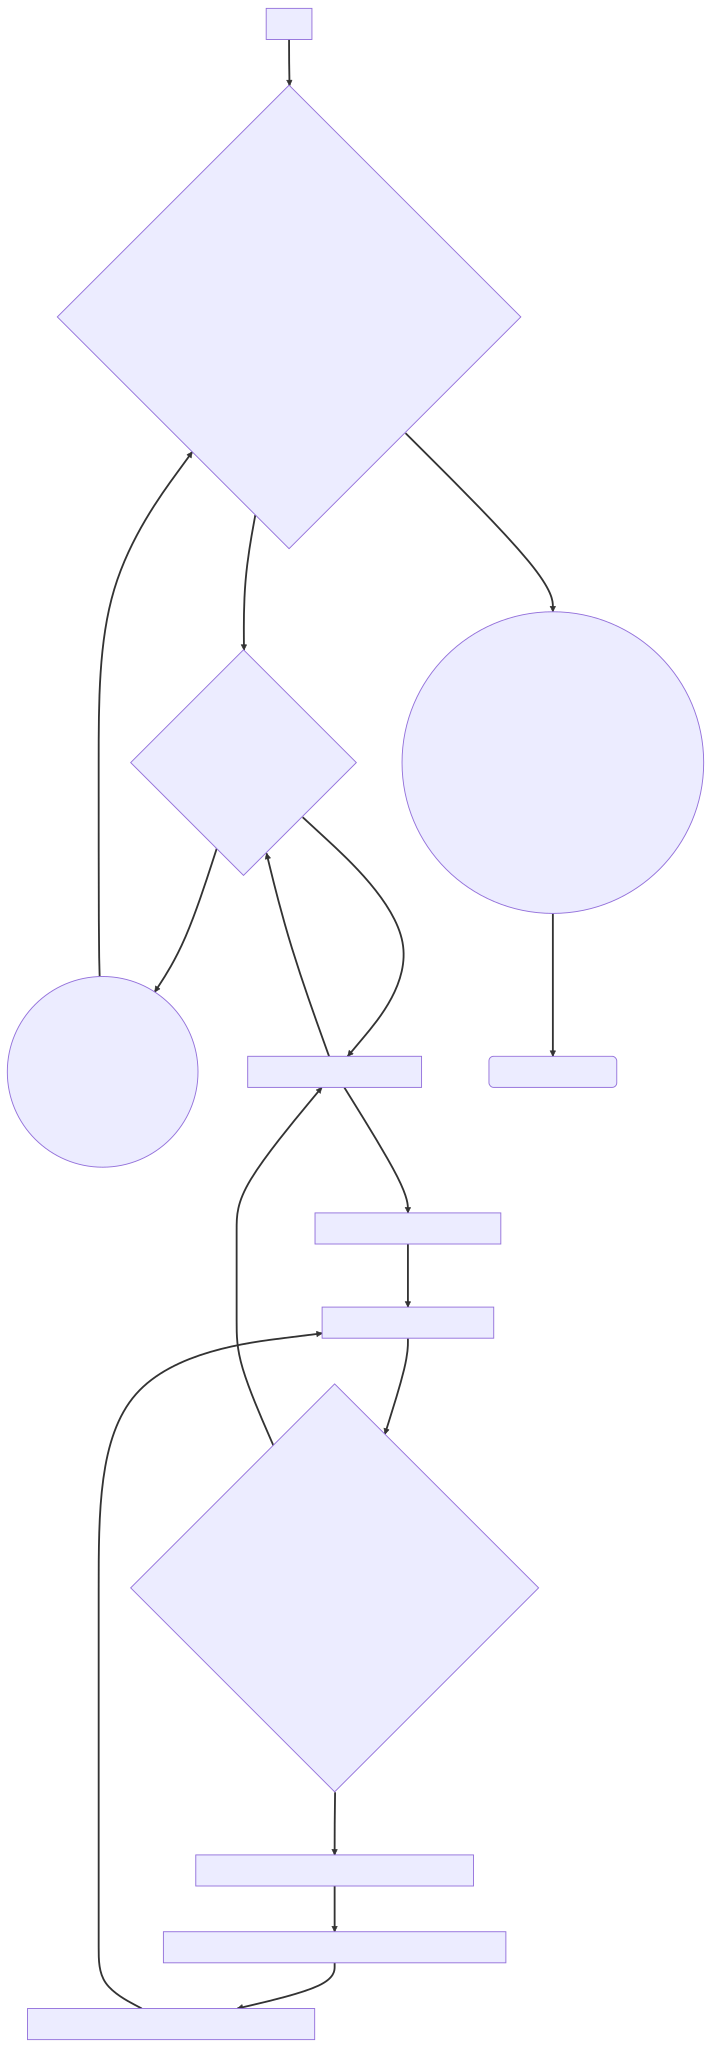
\includegraphics[width=0.8\textwidth]{images/batchsizefinder.pdf}
    \caption{Diagramatic representation of the Batch Size Finder Algorithm}
    \label{fig:bsfinder}
\end{figure}

\section{Result Aggregation} \label{sec:result_aggregation}
The biggest caveat of using Tensorboard is that the logs it generates cannot be directly queried in the interface itself. To overcome this, a custom script was written to query the logs and generate a DataFrame that combines all the logs into a single pandas DataFrame. This makes it possible to not only query the logs but also to perform any kind of analysis on them. This script can easily answer specific queries such as "What is the best accuracy across all the networks for 'gradcam++', 'dogs dataset' and 'proxy\_threshold = 0.5'?". This makes it possible to easily compare the performance of different models and configurations.

Since the script for aggregating logs is rather useful, it was made publicly available as a \href{https://gist.github.com/SubhadityaMukherjee/58cbdf324812175233e91993b720e0bc}{Github Gist}.

\section{Inference}
Inference refers to using a trained model to make predictions on new data. In this project, a large number of models were trained. A separate script was created to use any of the previously trained models for inference.\\
This script follows from the result aggregation and can use queries over the dataframe generated in the previous step. Since the generated dataframe also contains the path to the saved model, this script can use that information along with the names of the architecture, dataset and other hyper-parameters to load the required models easily.
The inference script also contains functions for comparing both the accuracies and the explainability of two pre-trained models given a validation dataset or a list of images.\\
For a batch of images and given a set of hyperparameters, the script loads two models - one trained with Proxy Attention and one trained without. The same dataloader is passed through both models to obtain predictions. Only EigenGradCAM is used for this evaluation phase to ensure a fair comparison, and since GradCAM++ was used for training, it would not be fair to use it for evaluation as well. \textcolor{red}{modify this a bit}

\textcolor{red}{\section{Auto-Generating the tables and plots for the report}}